% Preámbulo
\documentclass[stu, 12pt, letterpaper, donotrepeattitle, floatsintext, natbib]{apa7}
\usepackage[utf8]{inputenc}
\usepackage[T1]{fontenc}
\usepackage{adjustbox}
\usepackage{longtable}
\usepackage{tabularx}
\usepackage{lmodern}
\usepackage{comment}
\usepackage{marvosym}
\usepackage{graphicx}
\usepackage{float}
\usepackage[normalem]{ulem}
\usepackage[spanish]{babel}
\usepackage{multirow}
\usepackage{tabularx}
\usepackage{tabularray}
\usepackage{adjustbox}
\usepackage{geometry}
\usepackage{tikz}
\usepackage{enumitem}
\usepackage{hyperref}
\usepackage{amsmath}
\usepackage{pgfgantt}
\usepackage{apacite}
\usetikzlibrary{shapes.geometric, arrows, positioning}

\selectlanguage{spanish}
\useunder{\uline}{\ul}{}
\newcommand{\myparagraph}[1]{\paragraph{#1}\mbox{}\\}

% Portada
\title{\Large Informe de Resultados }
\author{
    Campero Morales José Antonio \\
    Campohermoso Berdeja Oscar \\
    Carrasco Cespedes Miguel Alejandro \\
    Martinez Acarapi Fabiola Alejandra \\
    Montero Garrido Diana Aneliz \\
    Zizold Sempertegui Gabriela Zulema Britta
}
\affiliation{Universidad Católica Boliviana}
\course{SIS-312: Gestión de Calidad de Sistemas}
\professor{Lic. Cecilia Alvarado Monrroy}
\duedate{\textbf{28 de octubre de 2024}}

\newcommand{\userstory}[5]{ % Change from 4 to 5 arguments
    \begin{center}
        \begin{tikzpicture}
            \node[draw, rounded corners, fill=blue!10, text width=0.9\textwidth, align=center, inner sep=10pt] {
                \textbf{#1} \\[5pt]
                \textit{Como} #2, \\[5pt]
                \textit{quiero} #3 \\[5pt]
                \textit{para} #4 \\[5pt]
                \href{#5}{Ver en GitHub} 
            };
        \end{tikzpicture}
    \end{center}
    \vspace{10pt}
}

\begin{document}
\thispagestyle{empty}

% Add the logo before the title content, avoiding extra space
\centering

\includegraphics[width=0.8\textwidth]{../imgs/logo-ucb.png} % Adjust the path to your logo image
\vspace{-5cm} % Adjust negative space if needed

\maketitle

% Índices
\newpage
\pagenumbering{roman}
% Contenido
\renewcommand\contentsname{\large Índice}
\tableofcontents
\setcounter{tocdepth}{2}
\newpage
% Fíguras
\renewcommand{\listfigurename}{\large Índice de figuras}
\listoffigures
\newpage
% Tablas
\renewcommand{\listtablename}{\large Índice de tablas}
\listoftables
\newpage

% Cuerpo
\pagenumbering{arabic}
\newpage
\section{\large Resumen de la prueba}
Durante el proceso de pruebas, se ejecutaron 42 casos de prueba que abarcaron las funcionalidades clave del sistema descritas en las 33 historias de usuario existentes. Del total de casos de prueba, 33 fueron aceptados sin observaciones, cumpliendo con los criterios de aceptación establecidos y asegurando el correcto funcionamiento esperado. Sin embargo, 9 casos fallaron debido a problemas encontrados durante la ejecución, los cuales fueron documentados y reportados para su resolución. 

A lo largo de las pruebas, se identificaron 28 defectos en los distintos módulos del sistema, estos se documentaron incluyedo detalles de reproducción, evidencias y sugerencias para su corrección, abarcando tanto aspectos funcionales como de accesibilidad. 

Además, se identificaron 7 alertas de accesibilidad, agrupadas según el criterio WCAG afectado, lo cual refleja la evaluación de la accesibilidad del sistema. 

\noindent Todos los reportes mencionados (Test Cases, reporte de errores y alertas de accesibilidad) se encuentran en los anexos.
\section{Reporte y Resultados}


\subsection{Resultados de las Métricas del Plan de Pruebas}

\noindent A continuación, se presentan las métricas recopiladas:

\begin{itemize}
    \item \textbf{Número de Test Cases ejecutados}: 7
    \item \textbf{Proporción de casos exitosos}: 42.86\% (3 casos pasaron, 4 fallaron)
    \item \textbf{Número de defectos identificados}: 4 (detallados en el reporte de defectos)
    \item \textbf{Tiempo total de ejecución de pruebas}: 15 horas-persona
    \item \textbf{Cobertura de Pruebas}: Se logró cubrir todas las funcionalidades según las historias de usuario, garantizando que las pruebas abarcaron la mayoría de las funcionalidades del producto. Esto asegura un monitoreo efectivo de la calidad de las pruebas y permite identificar áreas que podrían necesitar pruebas adicionales.
\end{itemize}

\begin{figure}[H]
    \label{fig:dashboard_metrica_pruebas}
    \centering
    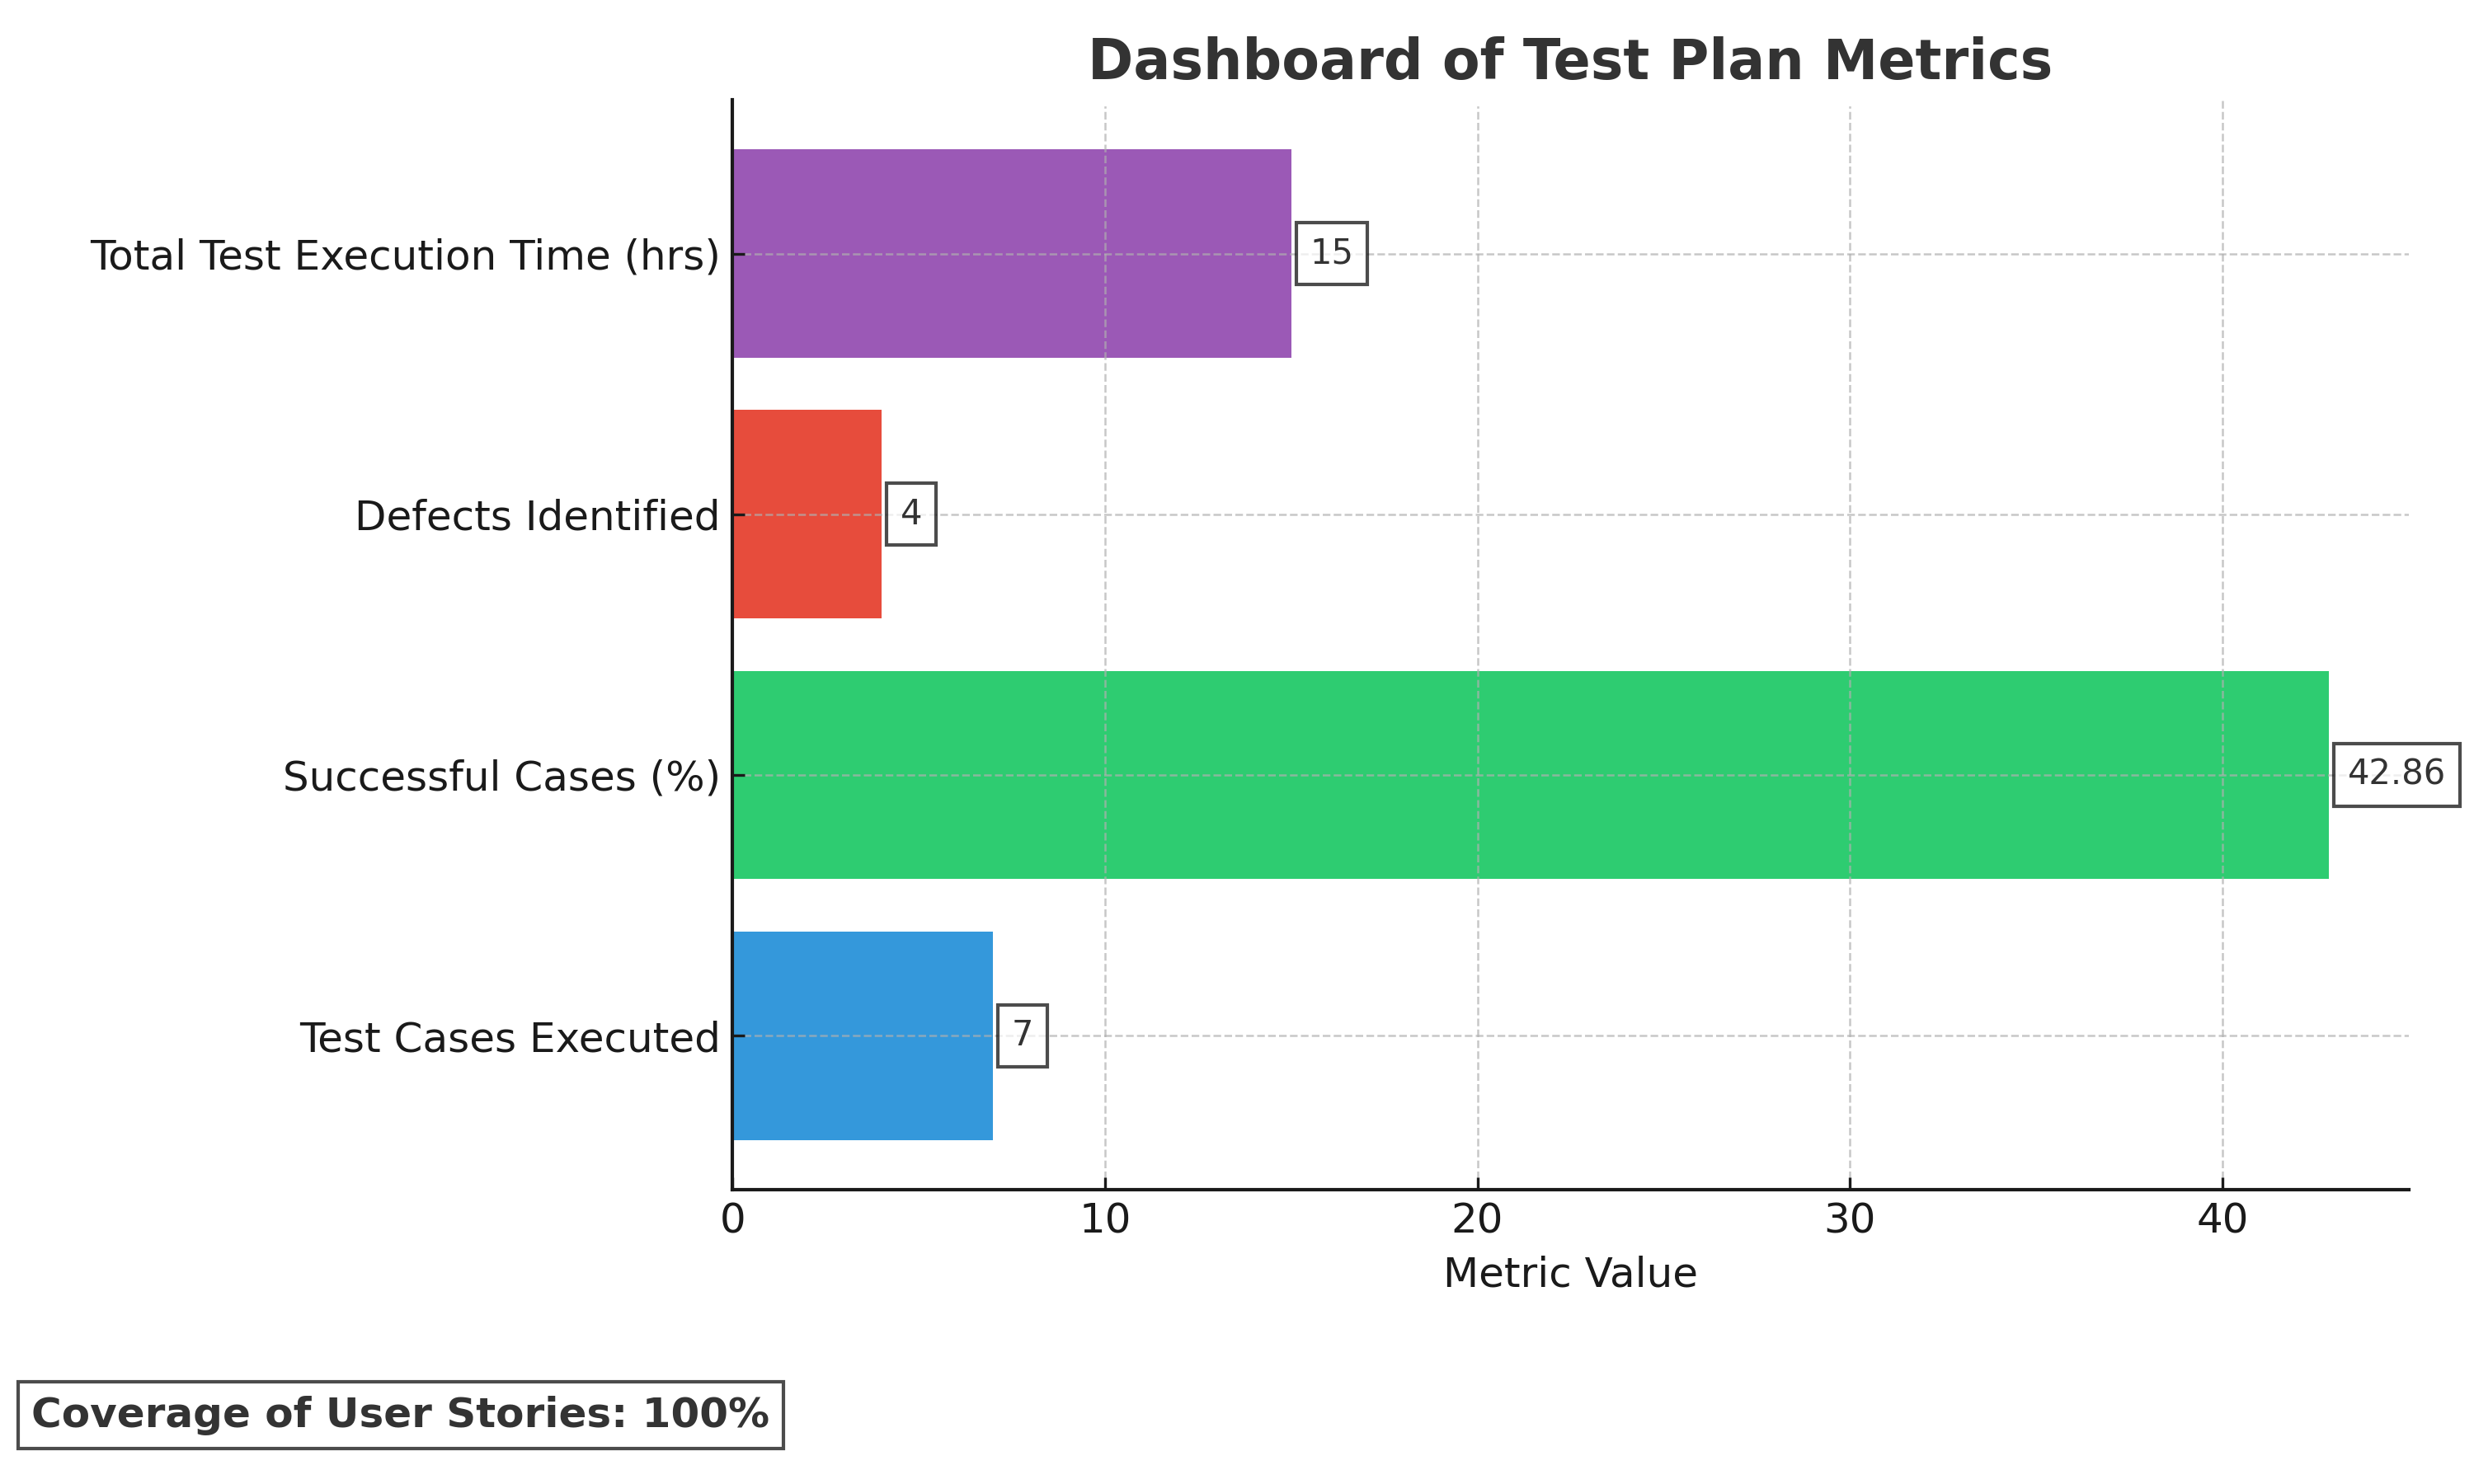
\includegraphics[width=\textwidth]{../imgs/dashboard_test_metrics_white_bg.png}
    \caption{Dashboard de Métricas del Plan de Pruebas}
\end{figure}

\section{Accesibilidad y usabilidad}

Las pruebas de accesibilidad realizadas con Axe DevTools revelaron varios problemas de accesibilidad, aunque en general, la cantidad de defectos encontrados no fue excesiva, lo cual es un indicio de que el sistema ya cuenta con una base relativamente sólida en términos de accesibilidad. Las pruebas que se llevaron a cabo se encuentran detalladas en el reporte de accesibilidad adjunto en anexos.
\subsection{Resultados Obtenidos en Pruebas de Usabilidad}

Las pruebas de usabilidad realizadas permitieron evaluar varios aspectos clave del sistema, como la visibilidad del estado, el control y la libertad del usuario, la consistencia y estándares, entre otros. En general, se detectaron áreas de mejora en términos de consistencia visual, retroalimentación al usuario, y navegación, los cuales se detallan en los resultados adjuntos. Cabe destacar que el sistema cumple con algunos de los principios fundamentales, como la flexibilidad y la visibilidad en varias de sus opciones, lo cual es positivo para la experiencia de usuario.

\noindent Para una descripción completa de los resultados obtenidos en cada ítem evaluado, por favor consulte los detalles (\hyperref[tab:reporte_usabilidad]{en Anexos})

\newpage
\section{Conclusiones}

\begin{itemize}
    \item \textbf{Evaluaci\'on general del sistema:} Los resultados obtenidos en las pruebas indican que el sistema cumple en gran medida con las funcionalidades especificadas, especialmente en los m\'odulos clave como los algoritmos Compet y Dijkstra. Sin embargo, tambi\'en se identificaron debilidades en la resistencia a casos at\'ipicos, accesibilidad y retroalimentaci\'on visual. Estas \'areas necesitan mejoras para garantizar un funcionamiento m\'as robusto y alineado con los est\'andares de calidad esperados.

    \item \textbf{Validaci\'on de datos y manejo de errores:} Durante las pruebas se detectaron defectos en la validaci\'on de campos obligatorios y num\'ericos, as\'i como en la notificaci\'on de errores en entradas inconsistentes. Estos problemas afectan la precisi\'on de los c\'alculos y la experiencia del usuario. La implementaci\'on de mecanismos de validaci\'on m\'as rigurosos y notificaciones espec\'ificas es esencial para corregir estas deficiencias.

    \item \textbf{Accesibilidad y usabilidad:} Las pruebas de accesibilidad revelaron incumplimientos con los criterios WCAG 2.2, como contraste inadecuado de colores y falta de etiquetado descriptivo para lectores de pantalla. Aunque se realizaron correcciones parciales, se recomienda implementar verificaciones recurrentes de accesibilidad para mejorar la experiencia de todos los usuarios, incluyendo aquellos con discapacidades.

    \item \textbf{Resultados de pruebas clave:} De los casos de prueba ejecutados, varios fueron aceptados sin observaciones, confirmando que los m\'odulos cumplen con los criterios de aceptaci\'on. Sin embargo, algunos defectos de baja prioridad y otros m\'as significativos, como problemas en la visualizaci\'on de listas extensas y superposiciones en el m\'odulo de Sorts, fueron documentados para futuras iteraciones.

    \item \textbf{Gestión de riesgos y defectos:} Se identificaron seis defectos importantes que, aunque no se corrigieron en su totalidad, han sido documentados detalladamente. La falta de ajustes autom\'aticos en situaciones de desbalance entre oferta y demanda tambi\'en representa un riesgo cr\'itico que debe priorizarse en las pr\'oximas fases de desarrollo.

    \item \textbf{Conclusión final:} Si bien el sistema demuestra estabilidad en sus m\'odulos principales y cumple con los requisitos funcionales, las \'areas de accesibilidad, usabilidad y documentaci\'on requieren atenci\'on significativa. Las mejoras sugeridas no solo aumentar\'an la calidad general del producto, sino que tambi\'en garantizar\'an una experiencia de usuario inclusiva y satisfactoria.
\end{itemize}

\section{Lecciones Aprendidas y Recomendaciones}

\begin{itemize}
    \item \textbf{Lecciones aprendidas:}
    \begin{itemize}
        \item La necesidad de pruebas tempranas y recurrentes en accesibilidad y usabilidad result\'o ser una lecci\'on clave para asegurar la inclusividad desde las etapas iniciales del desarrollo.
        \item La falta de estimaciones precisas en el tiempo necesario para la ejecuci\'on del plan de pruebas resalt\'o la importancia de una mejor gesti\'on de tiempos en proyectos futuros.
        \item La documentaci\'on limitada del proceso de desarrollo dificult\'o la replicabilidad de casos y la resoluci\'on eficiente de defectos.
    \end{itemize}

    \item \textbf{Recomendaciones para mejoras:}
    \begin{itemize}
        \item Implementar una suite de pruebas automatizadas para cubrir los endpoints y simplificar el testing continuo de la API.
        \item Mejorar el proceso de validaci\'on de datos, asegurando que todos los campos requeridos tengan validaciones adecuadas y mensajes de error comprensibles.
        \item Optimizar la accesibilidad mediante contrastes adecuados de colores, etiquetas descriptivas para lectores de pantalla y simplificaci\'on de la navegaci\'on.
        \item Realizar pruebas de carga y escalabilidad en m\'odulos como Sorts para asegurar el correcto funcionamiento con grandes vol\'umenes de datos.
        \item Priorizar la correcci\'on de defectos identificados en las pruebas, especialmente aquellos relacionados con accesibilidad y riesgos funcionales.
        \item Asegurar que futuras iteraciones incluyan documentaci\'on m\'as detallada tanto del proceso de desarrollo como del plan de pruebas, facilitando su comprensi\'on y mantenimiento.
    \end{itemize}
\end{itemize}



\newpage
\section{\large Anexos}

\subsection{Anexo A: Reporte de Defectos de Usabilidad} \label{tab:reporte_usabilidad}

\begin{longtable}{|>{\raggedright\arraybackslash}p{10cm}|>{\centering\arraybackslash}p{3cm}|}
    \caption{Plantilla de Reporte de Usabilidad} \label{tab:reporte_usabilidad} \\
    \hline
    \textbf{Items} & \textbf{Evaluation} \\ \hline
    
    \textbf{1.- Visibilidad del estado del sistema} & \\ \hline
    ¿Cada parte de la interfaz comienza con un título que describa el contenido de la pantalla? & Conforme \\ \hline
    ¿El diseño de íconos y su estética es consistente en todo el sistema? & Conforme \\ \hline
    Cuando se selecciona un icono que está rodeado de otros iconos, ¿Se distingue claramente el ícono seleccionado? & No Conforme \\ \hline
    Si se utilizan ventanas emergentes (pop-up) para mostrar mensajes de error, ¿Permiten esas ventanas que el usuario visualice el error en la interfaz cuando se despliegan? & No Conforme\\ \hline
    ¿Hay algún tipo de feedback para cada acción u operación? & No Conforme\\ \hline
    Luego de que el usuario completa una acción o serie de acciones, ¿El "feedback" del sistema indica que el siguiente grupo de acciones puede completarse? & No Conforme\\ \hline
    El sistema provee algún tipo de feedback visual en menús o cajas de diálogo que indiquen qué opciones pueden seleccionarse. & Conforme \\ \hline
    El sistema provee algún tipo de feedback visual en menús o cajas de diálogo que indiquen en cuál de las posibles opciones se halla posicionado el cursor. & No Conforme \\ \hline
    Si hay menús o caja de diálogo en donde pueden seleccionarse múltiples opciones, ¿El sistema provee algún tipo de "feedback" visual que indique cuáles son las opciones ya seleccionadas? & No Conforme \\ \hline
    ¿El sitio web entrega información corporativa de la organización? & Conforme \\ \hline
    Si existen demoras mayores a 15 segundos en las respuestas del sistema, ¿El usuario es informado del progreso en la concreción de la respuesta? & No Conforme \\ \hline
    ¿Informa datos relevantes para quien no "navega" (Ej: Horas de atención)? ¿Y para hacer consultas web o no web (Ej: números de teléfono)? & No Conforme \\ \hline
    ¿Los tiempos de respuesta son apropiados para cada tarea? & Conforme \\ \hline
    Tiempo de escritura, movimiento del cursor o selección con el ratón: entre 0,5 y 1,5 milisegundos & Conforme \\ \hline
    Tareas más comunes: 2 a 4 segundos & Conforme \\ \hline
    Tareas complejas: 8 a 12 segundos & Conforme \\ \hline
    No son necesarios altos niveles de concentración y no es requerido retener información: 2 a 15 segundos & No Conforme\\ \hline
    La terminología usada en los menús, ¿Es consistente con el dominio de conocimiento del usuario en relación a la tarea a realizar? & Conforme \\ \hline
    ¿El usuario conoce su ruta de ubicación? & Conforme \\ \hline
    
    \textbf{2.- Relación entre el sistema y el mundo real} & \\ \hline
    ¿Los íconos son concretos y familiares para el usuario? & Conforme \\ \hline
    ¿Los colores seleccionados corresponden a los valores esperados? & No Conforme \\ \hline
    Cuando se ingresan datos en la pantalla, ¿La terminología utilizada para describir la tarea es familiar para los usuarios? & Conforme \\ \hline
    Cuando la pantalla incluye preguntas, ¿El lenguaje de esas preguntas es claro y conciso? & N/A \\ \hline
    Las combinaciones de secuencias de letras o palabras extrañas o poco frecuentes, ¿Se evitan siempre que sea posible? & No Conforme\\ \hline
    El sistema ingresa/elimina de manera automática los signos de pesos o dólar y decimal cuando se insertan valores monetarios. & N/A\\ \hline
    ¿Se utilizan nombres unívocos y descriptivos en todo momento? & No Conforme \\ \hline
    ¿Se hace uso de los rastreadores de progreso? & No Conforme\\ \hline
    Los H1 están optimizados para SEO & No Conforme \\ \hline
    
    \textbf{3.- Control y libertad  por parte del usuario} & \\ \hline
    En sistemas que permitan el uso de ventanas superpuestas ¿Es fácil reacomodar reubicar esas ventanas en la pantalla? & Conforme \\ \hline
    En sistemas que permitan el uso de ventanas superpuestas ¿Es fácil para los usuarios cambiar de una ventana a otra? & Conforme \\ \hline
    Cuándo una tarea efectuada por el usuario se completa ¿el sistema espera alguna señal del usuario antes de procesar la tarea? & Conforme \\ \hline
    ¿Se pregunta al usuario que confime acciones que tendrán consecuencias drásticas, negativas o destructivas? & No Conforme \\ \hline
    ¿Existe una función para "deshacer" al nivel de cada acción simple, cada entrada de datos y cada grupo de acciones completadas? & No Conforme \\ \hline
    ¿Los usuarios pueden cancelar acciones en progreso? & No Conforme \\ \hline
    ¿Los usuarios pueden reducir el tiempo de entrada de datos copiando y modificando datos existentes? & Conforme \\ \hline
    Los menús son anchos (muchos ítems), antes que profundos (muchos niveles) & No Conforme \\ \hline
    Si el sistema posee menús de niveles múltiples ¿Existe algún mecanismo que permita a los usuarios regresar al menú previo? & Conforme \\ \hline
    Los usuarios pueden moverse hacia delante o hacia atrás entre las opciones de campos o cajas de dialogo. & Conforme \\ \hline
    Si el sistema utiliza una interfaz de preguntas y respuestas ¿Pueden los usuarios regresar a la pregunta anterior o saltear hacia delante una pregunta? & N/A \\ \hline
    ¿Los usuarios pueden revertir sus acciones de manera sencilla? & Conforme \\ \hline
    Si el sistema permite a los usuarios revertir sus acciones , ¿Existe un mecanismo que permita "deshacer" varias acciones de manera simultánea?  & No Conforme \\ \hline

    \textbf{4.- Consistencia y estándares} & \\ \hline
    El abuso de letras en mayúscula en la pantalla se ha evitado & No Conforme \\ \hline
    No hay más de 12/20 tipos de íconos & Conforme \\ \hline
    Existe algún elemento visual que identifique la ventana activa & Conforme \\ \hline
    Cada ventana posee un título & Conforme \\ \hline
    ¿Es posible utilizar las barras de desplazamiento horizontal y vertical en cada ventana? & Conforme \\ \hline
    Si una opción de un menú es la de "salir" ¿Esta opción aparece como ultimo ítem en el menú? & No Conforme \\ \hline
    ¿Los títulos de los menús están centrados o justificados a la izquierda? & No Conforme\\ \hline
    Fuentes: hasta tres tipos como máximo & No Conforme\\ \hline
    Hasta cuatro colores (usados ocacionalmente)  & No Conforme \\ \hline
    Sonido: tonos suaves para dispositivos de retroalimentación ocacional y bruscos para condiciones críticas. & N/A\\ \hline
    ¿Se provee una leyenda si los códigos de color son numeros o dificiles de interpretar?  & No Conforme \\ \hline
    Se evitan los pares de colores espectralmente extremos y altamente  cromáticos & No Conforme \\ \hline
    Los azules saturados no se utilizan para texto u otro elemento pequeño. & No Conforme \\ \hline
    La información más importante esta above the fold (la parte del sitio que los usuarios ven primero) & No Conforme \\ \hline
    ¿La estructura de la entrada de datos es consistente entre las diferentes pantallas? & No Conforme \\ \hline

    \textbf{5.- Prevención de errores} & \\ \hline
    ¿Las entradas de datos no son sensibles a mayúsculas siempre que sea posible? & No Conforme \\ \hline
    Las pantallas para entrada de datos y cajas de diálogo indican el número de espacios en caracteres que estan disponibles para un campo & No Conforme \\ \hline
    Los campos en las pantallas de entrada de datos y las cajas de diálogo ¿contienen valores por defecto cuando corresponden? & No Conforme \\ \hline

    \textbf{6.- Reconocer antes que recordar} & \\ \hline
    ¿Las áreas de texto tienen "espacios de respiración" que las rodeen? & No Conforme \\ \hline
    ¿Se ha utilizado el mismo color para agrupar elementos relacionados? & No Conforme \\ \hline
    ¿Existe buen contraste de brillo y de color entre los colores usados para imágines y fondos? & No Conforme \\ \hline
    Los colores suaves, brillantes y saturados se han utilizado para enfatizar datos, mientras que los colores oscuros, opacos y no saturados, han sido usados para des-enfatizar datos? & No Conforme \\ \hline
    ¿Los ítems inactivos en un menú aprecen en gris o están omitidos? & No Conforme \\ \hline

    \textbf{7.- Flexibilidad y eficiencia en el uso} & \\ \hline
    Los usuarios pueden reducir el tiempo de entrada de datos si se les permite copiar y pegar datos existentes. & Conforme \\ \hline
    Si las listas de menú son cortas (siete ítem o menos) ¿Pueden los usuarios seleccionar un ítem moviendo el cursor? & Conforme \\ \hline

    \textbf{8.- Diseño estético y minimalista} & \\ \hline
    Los íconos son visuamente distinguibles de acuerdo a su significado conceptual  & Conforme \\ \hline
    ¿Cada ícono esta resaltado con respecto a su fondo? & Conforme \\ \hline
    Cada pantalla de entrada de datos incluye un título simple, corto, claro y suficientemente distintivo. & No Conforme \\ \hline
    Los títulos de los menús son breves pero lo suficientemente largos como para comunicar su contenido. & No Conforme \\ \hline

    \textbf{9.- Ayuda a los usuarios a reconocer, diagnosticar y recuperarse de los errores} & \\ \hline
    ¿Los sonidos son utilizados para señalar errores? & N/A \\ \hline
    Si se usan mensajes de error con humor ¿Son apropiados y respetuosos para la comunidad de usuarios? & No Conforme\\ \hline
    ¿Los mensajes de error son gramaticalmente correctos? & Conforme \\ \hline
    ¿Los mensajes de error evitan el uso de signos de admiración? & No Conforme\\ \hline
    Los mensajes de error evitan el uso de palabras violentas u hostiles & No Conforme\\ \hline
    Si se detecta un error en un campo de entrada de datos ¿El sistema posiciona el cursor en ese campo o lo resalta de alguna manera? & No Conforme \\ \hline
    ¿Los mensajes de error sugieren la causa del problema que lo has ha ocacionado? & No Conforme \\ \hline
    ¿Los mensajes de error indican que acción debe realizar el usuario para corregir el error correspondiente? & No Conforme \\ \hline

    \textbf{10.- Ayuda y documentación} & \\ \hline
    ¿Las instrucciones en linea se distnguen visualmente?  & No Conforme \\ \hline
    Si las opciones de los menús son ambiguas ¿el sistema provee información aclaratoria adacional cuando un ítem es seleccionado? & No Conforme \\ \hline
    ¿La función de ayuda del menú es visible? (Por ejemplo una tecla etiquetada AYUDA o un menú especial) & No Conforme \\ \hline
    Navegación: la información es facíl de encontrar & Conforme \\ \hline
    ¿La información es exacta, completa y comprensible? ¿La información es relevante? & No Conforme \\ \hline
    Tras haber accedido a la ayuda ¿Pueden los usuarios continuar con su trabajo desde donde ha sido interrumpido? & Conforme \\ \hline
    ¿Es fácil acceder y regresar del sistema de ayuda? & Conforme \\ \hline
\end{longtable}

\end{document}
